% -*- root: These.tex -*-
\graphicspath{{FigureConclusion/}}

\chapter{Conclusion}

\startcontents[chapters]
\Mprintcontents
%%%%%%%%%%%%%%%%%%
% A RECASER : 

% Il ressortira de cette analyse toute la spécificité des sciences sociales et de la géographie, qui ne peuvent se satisfaire pour la construction de leurs modèles de simulation d'une vision de la « Validation » déracinée d'un contexte et d'une histoire des pratiques dans la discipline, car le modèle de simulation n'est qu'un type de modèles parmi les autres, souvent mobilisé dans un système de démarches plus complexes (Mathian and Sanders, 2014; Sanders, 2000; Cottineau, 2014)⁠. Ce n'est pas non plus dans l'usage de la modélisation multi-agents, ou d'une modélisation individu-centré plus « complexe à Valider » que niche cette problématique en géographie, mais bien dans l'adoption progressive d'un « projet systémique » (Pouvreau, 2013, page 9)⁠ accumulant et mobilisant les concepts, les méthodes et les outils mathématiques, statistiques et informatiques (Pumain, 2003)⁠ pour repenser la construction des modèles en tenant compte d'une « réalité » désormais comprise dans sa complexité. 

% Cette question de la « Validation » déjà en partie abordée dans ce débat clarifiant les acceptations du terme en fonction des disciplines, sera cette fois-ci déconstruit et mis de côté au profit d'une « évaluation »  (Amblard and Phan, 2006)⁠ dont on donnera les implications dans le cadre d'un objectif explicatif, en les plaçant au niveau d'une modélisation dont on a parfois tendance à oublier qu'il s'agit d'une activité de raisonnement scientifique avant d'être un modèle aplani et lissé de toutes ses aspérités (Langlois and Reguer, 2005, page 36)⁠.  

%%%%%%%%%%%%%%%%%%

% Présentation limites des méthodologies existantes
% Proposition d'une grille générique de lecture

Dans le dernier chapitre de cette thèse, consacré à la description du framework MGO, nous avons montré qu'il était possible d'offrir une première construction d'intégration pour la plateforme OpenMOLE qui soit à la fois bénéfique aux modélisateurs géographes, mais aussi de façon plus générale à l'ensemble des modélisateurs de la communauté des systèmes complexes. Afin de bien situer ce résultat principal de notre travail dans une littérature en constant mouvement et très interactive, il nous semble important de rappeler qu'elles sont les options choisies par d'autres réalisateurs de plateformes, ce qui permet de mieux évaluer ensuite la pertinence des principes que nous avons suivis.

Dans cette conclusion, nous rappelons donc quelques insuffisances liées aux méthodes de modélisations existantes qui sont un des résultats saillants de nos recherches sur les racines de cette histoire et de notre veille sur la littérature pluridisciplinaire associée, avant de résumer notre grille de principes à mettre en oeuvre pour la construction d'une double plateforme, en accord avec les remarques théoriques faites sur l'évaluation dans la partie 1 : une plateforme pour la construction de modèle et une plateforme pour l'exploration des modèles. Cette grille nous permettra également de fixer un horizon d'amélioration pour les projets déjà en cours dans cette équipe. 

\section{L'insuffisance des méthodes existantes}
\label{sec:insuffisance_plateformes}

\subsection{Le \textit{BehaviorSearch} et le \textit{BehaviorSpace} de Netlogo}

Une initiative remarquée est celle menée depuis plusieurs années par l'équipe de Wilensky, connu principalement pour avoir développé le simulateur Netlogo. Parmi les publications écrites par Wilensky plusieurs mettent en avant \autocite{Wilensky2007a} - comme d'autres l'ont également fait dans la communauté Agents \autocites{Rouchier2013, Axtell1996} - l'importance de \enquote{pratiquer la reproductibilité} pour nous et pour les autres. Un des objectifs visés étant la constitution d'une communauté scientifique capable de dégager de nouveaux savoirs par le partage et la discussion collective des modèles. Une recette que Wilensky a appliquée avec succès dans la reproduction de nombreux modèles afin de les faire figurer dans sa plateforme, et qu'il faut évidemment mettre en perspective des principaux traits faisant toute la valeur du simulateur Netlogo. 

Avec Stonedahl \autocites{Stonedahl2011, Stonedahl2011b, Stonedahl2010} il explore cette fois-ci une autre dimension de la validation en s'attaquant à l'exploration automatique des modèles de simulation écrits en Netlogo. L'outil \textit{Behavior Search} ainsi développé par \textcite{Stonedahl2011a} s'appuie sur des méta-heuristiques, principalement de la famille des Algorithmes Evolutionnaires (EA). Cet outil se place volontairement dans la continuité de l'\enquote{esprit Netlogo}\Anote{stonedahl_netlogo}, à savoir offrir des outils à la fois suffisamment simples d'accès pour s'adapter à un public \enquote{débutant en modélisation}, tout en étant suffisamment complets, évolutifs, pour intéresser et accompagner les recherches d'un public essentiellement scientifique. Les outils accèdent avec leurs diffusions à un niveau de standardisation qui leur permet de toucher à cette dimension sociale constitutive d'une partie de la validation.

L'accroche d'un public aux compétences variables, qu'ils soient experts ou débutants, fait souvent partie des enjeux dans la création d'une nouvelle plateforme pour la modélisation. La plus ancienne des librairies multi-agents \textit{Swarm} était déjà pensée par Langton comme une étape supplémentaire vers la démocratisation des outils. Un saut qui a permis de fédérer une première communauté, mais qui n'était pas suffisant pour toucher un public de non-programmeurs. Netlogo, le jumeau scientifique de la plateforme StarLogo dédiée aux enfants, a permis ces dernières années de redonner une part d'autonomie aux chercheurs des sciences sociales dans la manipulation de leur objet de recherche. Pour \textcite{Banos2013}, cet outil permet de concrétiser à moindre coût et de façon quasi instinctive le contenu des discussions scientifiques dans un modèle exécutable tangible. Il en ressort un véritable outil d'accompagnement de la pensée scientifique, qui permet de concrétiser et de communiquer une idée au travers d'un modèle dans un temps record. On se rapproche ici d'un système où le coût d'entrée est très faible par rapport aux gains supposés, le langage étant volontairement limité dans le nombre de primitives disponibles, celui-ci est rapidement assimilable, même pour des non programmeurs. 

Mais, si Netlogo répond de façon parfaite à cette nécessité de prototypage rapide et peu couteux, un scénario tout à fait adapté pour découvrir la modélisation, il ne permet pas par contre de répondre à un scénario pourtant classique rencontré par les modélisateurs souhaitant faire évoluer leur modèle sur le temps long au-delà d'une certaine complexité. Ainsi, tant d'un point de vue algorithmique, que du point de vue des ressources informatiques nécessaires à l'exécution et à l'évaluation de modèles, Netlogo ne permet pas de supporter une montée en complexité pourtant naturelle dans le cadre de tels projets. 

On sait également que la diversité et la complémentarité des approches sont un point central dans l'étude des systèmes complexes; or si Netlogo donne effectivement à voir cette diversité par la présence d'une large bibliothèque de modèles, celle-ci n'est abordée que dans une seule dimension, celle du modèle, et sous un seul format, celui de Netlogo. Or chacune des disciplines dispose de ses propres outils, de ses propres formalismes, de ses propres formats que Netlogo serait bien en peine de vouloir reproduire à l'identique. Cette diversité d'approche caractéristique des systèmes complexes dépasse qui plus est largement largement le cadre de la seule description du modèle et touche également l'environnement qui gravite autour de lui. Choisir Netlogo c'est prendre le parti d'un formalisme qui donne accès à une communauté, à un ensemble d'outils, mais qui ne permet pas d'exploiter au mieux les apports de diversité propre aux pratiques de modélisation de chacune des disciplines. 

La librairie \textit{BehaviorSearch} développée par Stonedahl pour Netlogo intègre une librairie d'algorithmes génétiques. Cette solution n'est pas entièrement satisfaisante du seul point de vue avancé des métaheuristiques :
\begin{itemize}
\item Le cycle de vie d'un modèle ne se limite pas forcément à l'établissement d'un seul modèle Netlogo, mais plusieurs, et de complexité différente. Si Netlogo est un outil indispensable de par la force et la rapidité de concrétisation d'une idée scientifique qu'il permet, les scientifiques auto-didactes peuvent rapidement être piégés par des problématiques tenant plus de la \enquote{science informatique} que de leur domaine initial.

\item Le niveau de prise en charge de l'expérimentation est insuffisant pour assurer une recherche reproductible au-delà du seul modèle. Par là il faut comprendre que le protocole scientifique supportant l'évaluation du modèle de simulation n'est pas accessible, or tout comme le modèle, celui-ci possède sa propre voie de construction, et porte au contact du premier une responsabilité dans l'évolution des choix de sa structure interne. Autrement dit, sans la présence de ces deux supports de connaissances, c'est toute une discussion collective qui est rendue plus difficile, alors même que celle-ci se révèle comme un support important, voire même constitutif de ce processus de validation.

\item Le support du parallélisme implicite à ce type de métaheuristique EA en local, c'est-à-dire sur un ordinateur personnel, même lorsqu'il est associé à des techniques pour réduire le nombre d'exécutions des modèles de simulation (en utilisant par exemple du \textit{fitness caching} \autocite[245]{Stonedahl2011a}), ne semble pas suffisants pour une utilisation confortable et répétée d'algorithmes métaheuristiques multi-objectifs. Ces derniers pouvant demander pour des modèles relativement simples et optimisés jusqu'à plusieurs millions d'exécutions, résultat d'une accumulation d'expérimentation nécessaire pour la construction et l'évaluation du modèle de simulation \autocites{Schmitt2014, Cottineau2014b}. Le framework théorique QBME (\textit{Query-Based Model Exploration}) de Stonedhal est intéressant, et ressemble par certains aspects à la méthodologie POM de Grimm, il permet comme dans cette dernière de questionner la progression du modèle sous la forme d'une question inversée par rapport au questionnement plus traditionnel. On ne se demande plus \enquote{Quels comportements vais-je obtenir avec ce jeu de paramètres} mais plutôt \enquote{Quels types de paramètres m'a permis d'obtenir (ou de ne pas obtenir) un certain comportement ?} Ce type d'analyse se base sur la construction de multiples critères d'évaluation, potentiellement contradictoires, questionnant la dynamique du modèle, et qui il me semble, se rattache plus à l'expression d'une analyse multi-objectifs. Or, les algorithmes proposés par le \textit{BehaviorSearch} se limitent pour le moment à des algorithmes mono-objectifs que les cas d'utilisation réels risquent de très rapidement mettre en défaut.

\item Le support ne permet pas à l'heure actuelle de jouer \enquote{facilement} avec les briques mises à disposition par les métaheuristiques, ce qui on l'a vu précédemment va à l'encontre de l'esprit de tels algorithmes. Même si une certaine extensibilité du logiciel a été prévue par le concepteur, sa mise en oeuvre demande des connaissances supplémentaires dans un autre langage de programmation que Netlogo (Scala ou Java), ce qui vient encore surcharger un peu plus les prérequis d'un utilisateur débutant qui doit déjà explorer le domaine des algorithmes évolutionnaires.
\end{itemize}

Même si on peut être est effectivement d'accord avec le concepteur du \textit{BehaviorSearch} pour dire que cet outil constitue en lui même déjà un grand pas vers la démocratisation de techniques d'expérimentation plus évoluées jugées nécessaire pour améliorer les pratiques des débutants, nous pensons qu'il est possible d'aller encore beaucoup plus loin. A ce titre, le couplage que nous visons dans ce projet se rapproche des visions d'avenir évoquée par le concepteur, dont la dernière version du logiciel est datée de 2013 \textcite[295]{Stonedahl2011a} \foreignquote{english}{In the not-so-distant future I envision in a “begin parallel search” button appearing in toolkits like NetLogo that would seamlessly launch dozens or hundreds of simultaneous genetic algorithms searches on a remote grid/cluster, reporting back the most promising results to the user as they are discovered in real-time.} La différence c'est que ce bouton n'est pas envisagé dans Netlogo, car ce n'est pas le propre de cet outil, mais dans un logiciel tel qu'OpenMOLE, dont la fonction est entièrement dédiée à l'exécution de tâches en parallèle sur des environnements locaux (un ou plusieurs processeurs d'une machine), ou distribués (sur une grille de calcul, ou un cluster d'université)

Si on envisage en effet la construction de modèles sur la base d'une alternance régulière entre construction de modèles et évaluation, il est tout à fait possible et même certain que l'expérimentateur soit un jour ou l'autre confronté à une ou plusieurs limitations provenant de la chaîne de progression naturelle prévue par les concepteurs de cet outil \foreignquote{english}{Netlogo(for building the model) => Behavior Space (for simple model analysis) => BehaviorSearch (for more advanced analysis and exploration)} \autocite[340]{Stonedahl2011a} 

En résumé, les librairies déjà intégrées au logiciel de modélisation, comme le \textit{BehaviorSearch} de Netlogo, sont limitées en termes d'algorithmes, d'accès la puissance informatique nécessaire, et reste liées à un seul et unique support alors même que le modèle peut être amené à migrer de plateforme. On en déduit que cette solution, bien qu'utile pour du prototypage et de l'apprentissage, ne permet pas d'envisager sereinement la construction d'un modèle ou d'une expérimentation sur une durée plus longue.

\subsection{Mason et ses algorithmes EC}

Le framework de développement de simulation multi-agents MASON (\textit{Multi-Agent Simulation Of ...}) présenté pour la première fois en 2003 tient d'un effort conjoint entre la section d'\textit{Evolutionary Computation} du laboratoire de science informatique et le \textit{Center for Social Complexity} tout deux de la George Mason University. Ecrit en Java, solidement documenté, de développement ancien, associé depuis les débuts à un laboratoire spécialisé auteur d'une librairie datant de 1998 dédiée aux EC nommée ECJ (1998), les deux logiciels étant développés par les mêmes personnes et régulièrement mis à jour ... ce framework apparait au premier abord comme un challenger sérieux pouvant se substituer à Netlogo sur des projets plus complexes.

MASON se situe sur la même ligne de développement que les librairies de développement multi-agents plus anciennes comme Swarm, Ascape, ou Repast. Tout comme ces dernières, la généricité, la performance et la modularité sont des composantes de l'application au coeur des préoccupations de Sean Luke, un des développeurs à l'origine du projet.

Une des spécificités très fortes de MASON, et qui rend cette librairie vraiment différente des trois autres, tient dans son histoire particulière. Si on en croit le développeur Sean Luke \Anote{sean_luke_mason}, c'est à la suite de sa thèse en 1998 et du développement de la librairie ECJ \Anote{sean_luke_ecj} dédié aux algorithmes d'EC, que celui-ci a ressenti le besoin d'une nouvelle librairie en accord avec ses problématiques de recherches en robotiques. A cette époque déjà, il utilise ECJ pour optimiser le comportement de robots opérant dans un environnement partagé, un domaine de recherche très proche de la simulation multi-agents \enquote{réactive} historiquement \autocites{Brooks1991, Steels, Ferber}. Cette pratique nécessite l'exécution de centaines de milliers de simulations, à la recherche de combinaisons de paramètres satisfaisant les critères dirigeant l'optimisation. La rapidité d'exécution d'une simulation devient un élément clef dès lors que ce sont des milliers, voire des millions de simulations qui doivent être executées en parallèle. C'est donc tout naturellement que celui-ci a initié sa propre librairie de simulation multi-agent, orientée vers l'utilisation efficiente des architectures multi-coeurs et depuis peu multi-ordinateurs (extension D-Mason). MASON étant conçu en parallèle de la librairie \href{http://cs.gmu.edu/~eclab/projects/ecj/}{@ECJ}, les deux outils fonctionnent très bien ensemble, et permettent l'exploitation de ressources informatiques dans des environnements distribués, initialement des clusters \autocite[211]{Luke2014}, bien qu'une \href{http://www.parabon.com/dev-center/origin}{@extension} apparemment payante permette de faire du \textit{Grid Computing}.

ECJ ou Mason sont des outils à destination de développeurs spécialistes lorsqu'il s'agit de coupler les deux outils. Ce point de vue est délibérement assumé par l'auteur dans le manuel de MASON \Anote{sean_luke_masondifficile}, et ECJ \Anote{sean_luke_ecjdifficile}.

Il est toutefois intéressant de voir que malgré des optiques de développements différentes et une réalisation inverse à la nôtre, l'objectif motivant la construction est le même, mettre à disposition des ressources informatiques nécessaires à l'utilisation de méta-heuristiques pour l'évaluation de modèles de simulation. En effet, là où Luke justifie d'un nouveau framework agent pour rendre efficiente l'utilisation de sa librairie d'EC, c'est pour nous la démarche inverse qui prime, et c'est la nécessité d'intégrer l'optimisation comme pratique standard dans la construction d'un modèle qui justifie d'un framework EC adapté. Les deux approches sont complémentaires, et cette question de l'efficience légitime tout à fait un changement de support de modélisation dès lors qu'on essaye de complexifier les modèles. Car comment évaluer un modèle de simulation dont une seule des exécutions dure plusieurs heures ? Notre approche se veut toutefois plus respectueuse des pratiques existantes, et la réalisation support de l'exploration du modèle, une fois mise en oeuvre, doit concéder aux utilisateurs la même facilité d'accès aux EC, qu'ils utilisent Netlogo, Mason, ou une plateforme de leur initiative.

\subsection{Une analyse critique de la méthodologie moderne POM}
\label{ssec:critique_pom}

%que sur  celle ci ne doit pas être  relativement peu de méthodologie clef en main qui s'attaque de front à cette problématique, la plupart se bornant seulement à l'établissement de guides de bonne pratiques, ou de listes d'outils (mathématiques, statistiques, informatiques) disponible.

Ces dernières années l'équipe d'écologues réunis autour de Volker Grimm est très certainement celle qui milite le plus activement pour une formalisation des pratiques dans la communauté de modélisateurs. En dehors des publications et ouvrages ayant marqué depuis des décennies cette communauté de modélisateurs individu-centré en écologie \autocites{Huston1988,DeAngelis1992,Grimm1999,Grimm2004,DeAngelis2014}, plusieurs propositions ont également été faite plus récemment, à destination de la communauté de modélisateurs au sens large. Il y a d'abord eu en 2006 d'un protocole de description de modèle multi-agents nommé \textit{Overview, Design concepts, and Details} (ODD) \autocite{Grimm2010}, puis la méthodologie de construction de modèles de simulation dite de \textit{Pattern Oriented Modelling} (POM) \autocites{Grimm2005}. Cette méthodologie a trouvé en 2012 une instanciation très concrète dans l'excellent ouvrage d'introduction à la modélisation agents à destination des débutants de \textcite{Railsback2012}, qui s'appuie largement sur Netlogo. La méthodologie POM a même été reprise de façon explicite par des géographes en pointe sur la simulation appliquée au spatial, et les problématiques d'équifinalité/multi-modélisation \autocite{OSullivan2004, Millington2012}. Ces travaux présentés dans l'ouvrage de \textcite{OSullivan2013} sont là aussi exemplifiés avec Netlogo. Cette équipe s'est attaquée plus récemment à l'absence d'outils et de revue de littérature sur les analyses de sensibilités \autocites{Thiele2012,Thiele2014}, alors même que celles-ci sont reconnues depuis des décennies comme des techniques essentielles et absolument nécessaires pour construire des modèles de simulation. Enfin, c'est pour régler la confusion qui règne autour des termes de Validation en écologie (mais pas seulement) que l'équipe de Grimm propose un nouveau terme d'\enquote{évaludation} contractant Validation et évaluation \autocite{Augusiak2014}. 

Comme le disent très bien \textcite{Railsback2012} dans leur définition de POM \Anote{railsback_POM_resume}, cette stratégie pour la construction de modèle ne fait qu'expliciter une méthodologie la plus souvent déjà opérante chez des scientifiques modélisateurs expérimentés. Toutefois, le transfert de cet implicite dans une méthodologie bien nommée offre au-delà d'un acronyme la possibilité d'une mise en avant de ce processus \enquote{constitutif du modèle} qu'est l'activité de construction (voir \ref{p:autre_def_modele} et le chapitre précédent), une activité pour laquelle on n'accorde encore que peu d'importance dans l'écriture des publications, souvent au seul profit des résultats. A la différence de la démarche KISS (\textit{Keep It Simple Stupid}), parfois reprise par les auteurs de modèles de simulation comme un argument suffisant pour justifier d'une construction, POM va à mon sens beaucoup plus loin. D'une part, car celle-ci donne à voir un outillage conceptuel beaucoup plus concret pour encadrer, diriger la construction de modèles, et d'autre part, car elle met ce processus en regard de l'élaboration de \textit{patterns}, des critères qualitatifs ou quantitatifs utilisés à la fois comme heuristique pour intégrer des éléments échappant au modèle conceptuel initial, mais également comme filtre permettant de justifier l'organisation interne retenue dans nos constructions. Ainsi, on retrouve dans l'argumentation de Railsback et Grimm cette idée d'élaboration d'une évaluation multi-critères guidée par l'apport cumulatif de crédibilité qu'elle permet sur le réseau d'hypothèses du modèle, un constat déjà esquissé par Hermann à la fin des années 1960 et dont nous avons déjà analysé l'importance dans la section \ref{ssec:evaluation_construction}. 

%10:32 <Skizomeuh> RT @_FabV: [81] Un nouveau long-métrage Ghost in the Shell prévu pour l'été prochain, par l'équipe de ARISE https://t.co/tOnztTF0aA http://t.co/V1SqWwjEZV
% Timur Vermes, un livre énorme ! A lire ab-so-lu-ment !
% RT @GrapheneDB: [52] Popoto.js a graph search generator JS lib for the @neo4j #graphdb, by @FredCiminera - http://t.co/gn85K2kjYG
% http://t.co/5gjkzz8K08

La première étape de POM intitulée \foreignquote{english}{Pattern for model structure} s'appuie sur l'expertise des chercheurs spécialistes du domaine pour établir la partie \foreignquote{english}{Overview} de la feuille de route ODD : identifier l'objectif motivant le modèle, les entités, les variables, les dynamiques, l'enchainement général du programme, les \textit{patterns}, et les critères de mesure pour ces \textit{patterns} que l'on estime nécessaire pour la construction d'un premier modèle \textit{a priori} capable de faire \enquote{émerger} les \textit{patterns} retenus. La selection des \textit{patterns} permet de fixer outre la limite posée par l'établissement d'un modèle conceptuel, une autre limite qui se rapporte celle-ci à la richesse de la structure interne du modèle. L'objectif de ce processus étant de se trouver à l'équilibre dans ce que les écologues appellent une \foreignquote{english}{Medawar zone}, calculé comme étant l'optimum entre \enquote{la position la plus avantageuse d'un point de vue des connaissances extraites} (\textit{payoff}) et sa \enquote{complexité de mise en oeuvre} (\textit{difficulty}). Il est évident que seul un modèle de simulation opérationel permet de se positionner dans une telle zone. \Anote{railsback_POM_structure}

L'étape suivante invite donc les modélisateurs, si ce n'est pas déjà fait, à construire un premier modèle fonctionnel, même incomplet, afin d'entrer le plus vite possible dans l'étape dite de \foreignquote{english}{theory development} visant l'amélioration incrémentale du modèle.

La \enquote{dé-simplification} ciblée du premier modèle opérationel passe par la formulation d'hypothèse alternatives (\foreignquote{english}{alternative hypotheses} ou \foreignquote{english}{traits}) spécifique des comportements agents (\foreignquote{english}{agents behaviors}) que l'on veut observer dans le modèle. \Anote{agent_grimm} 

% Ajouter le fait que Sullivan cite aussi cette expression.
La stratégie \foreignquote{english}{null theories} \Anote{railsback_POM_nulltheories}  consiste à implémenter pour chacun des comportements d'agent amenés à varier par la suite, une version ne faisant appel si possible à aucune théorie particulière, minimisant de fait l'impact interpretatif du modèle initial. En résumé l'objectif est de pouvoir quantifier dans un premier temps et par rapport au critère renseignant l'émergence des \textit{patterns}, quel est le poids interprétatif attribuable à la structure du modèle ainsi mis à nu, puis d'observer dans un deuxième temps, dans l'évolution du modèle et des hypothèses, quel est l'apport exact de chaque nouveau comportement implémenté sur la dynamique générale du modèle.

Pour Grimm, c'est dans cette activité ou les modèles agents endossent pleinement le rôle de \enquote{laboratoire virtuel} que s'exerce véritablement l'activité de raisonnement scientifique. Le modélisateur est amené à exercer son talent de détective via tous les moyens classiques de l'entreprise scientifique, cela dans le but d'imaginer, d'implémenter puis de juger par la mise en concurrence et l'évaluation de paramètres et d'hypothèses alternatives le modèle le plus à même de reproduire les \textit{patterns} retenus jusqu'alors. 

Il est tout à fait possible de voir le dialogue qui peut s'instaurer entre ces deux grandes étapes, la structure initiale très simple du modèle s'adaptant progressivement et de façon conséquente aux résultats tirés de l'analyse confrontant \textit{patterns} et données résultats du modèle. Une confrontation dont l'analyse permet de voir émerger non seulement la formulation de nouvelle hypothèses, mais également la modification ou la création de nouveau critères, et patterns. Ce cycle est très bien illustré par la figure \ref{fig:S_syntheseGrim} de \textcite{Railsback2012}.

\begin{figure}[h]
\begin{sidecaption}[fortoc]{ POM cycle for developping theory for an agent behavior \autocite[245]{Railsback2012}}[fig:S_syntheseGrim]
  \centering
 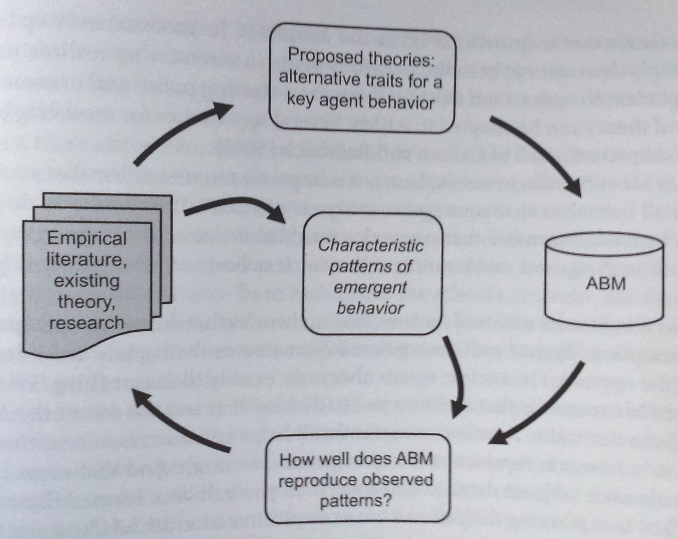
\includegraphics[width=.9\linewidth]{cyclePOMcomportement.png}
  \end{sidecaption}
\end{figure}

L'analyse est une étape qui porte la compréhension du modèle, et nous sommes en accord avec Grimm pour dire que celle-ci est indissociable de la construction du modèle, et doit être mise en oeuvre le plus tôt possible, dès que celui-ci s'avère fonctionel. \enquote{Sinon comment justifier de la connaissance produite avec un modèle de simulation ?} Cette question renvoie aux réflexions épistémologiques et philosophiques citées dans la section \ref{ssec:evaluation_construction}. Le fait que le modèle de simulation s'exécute ici sur un substrat artificiel détaché de toute réalité physique est depuis longtemps reconnu comme un des arguments favoris des détracteurs de la simulation. Bien que reconnu comme assez ancien, cet argument montre par sa présence encore aujourd'hui dans l'argumentaire de certains auteurs et certaines disciplines, qu'il est important de montrer à quel point les modélisateurs apportent un soin à faire de ce transfert des conclusions des modèles à la réalité une affaire prudente. % Cf appel réf monde crédible dans le chapitre précédent ?

La qualité, la disponibilité et la reproductibilité du modèle, et du raisonnement qui lui ont donné naissance deviennent alors des pré-requis absolument nécessaires pour parer à toutes critiques concernant la scientificité des résultats apportés par ce type de modélisation. % qu'il s'éloigne finalement assez peu des techniques déjà mis en oeuvre pour la construction de modèle de simulations équationels, .

Car comment peut on faire état d'un transfert possible de connaissance à la réalité si l'étape préalable qui consiste à analyser les comportements du modèle n'est pas réalisée ? Comment justifier de la construction d'un modèle dont on ne mesure pas son fonctionnement interne à l'aune des critères dont on dispose pour caractériser la réalité dont on veut rendre compte ?

L'approche de Grimm et Railsback constitue à bien des égards une véritable avancée pédagogique, de par sa double implication méthodologique et technique. Les débutants ont a leur disposition un support de résolution (Netlogo), un véritable objectifs à atteindre (\textit{Patterns}), et surtout, ce qui manque à la plupart des guides, une méthodologie de construction concrète et exemplifiée (POM).

Mais, si elle met bien en valeur l'importance de cette activité de raisonnement qu'est la deconstruction, reconstruction des hypothèses et des critères du modèle, Grimm oublie il me semble de poser une question importante qui nécessite de rentrer un peu plus dans ce processus de construction. % pour la crédibilité d'un raisonnement aussi linéaire dès lors qu'on est confronté à un vaste réseau d'hypothèse.

Comme le décrit Grimm, les \textit{patterns} jouent le rôle de support heuristique accompagnant l'apparition des entités ou des processus que nous n'aurions justement pas pensé à injecter dans le modèle en première analyse. Il est alors évident que ce processus nécessite une grande plasticité dans la formation des hypothèses alternatives, dont le niveau d'abstraction et de formalisation n'est en aucun cas homogène, au contraire. Or Grimm ne dissocie l'hypothèse de sa traduction informatique que sur des exemples très simples. Mais notre expérience acquise en modélisation a montré que la variabilité introduite dans ce processus est double, et peut apparaitre à la fois au niveau de la traduction informatique d'une seule et même hypothèse, tout autant que dans sa formulation alternative. Ces deux interventions peuvent rapidement impacter tout ou partie des éléments déjà mis en place, que cela soit au niveau conceptuel et, ou informatique. On peut pour donner un exemple, se poser la question de la définition des modalités d'un marché régissant les échanges au niveau de chaque ville dans un système de villes pour donner un aperçu de la multiplicité d'hypothèses et d'échelles qui peuvent être envisagées lors de sa traduction informatique, et cela sans compter la combinatoire qui en résulte : définition de la portée des échanges ? stratégies régissants les échanges ? influences environnementales ? etc. Cette hypothèse ouvre, même en restant dans une optique parcimonieuse, vers une multiplicité de sous-modèles et d'hypothèses alternatives dont l'implémentation appelle forcément la création ou la modification d'autres entités et d'autres processus. Autrement dit, il y'a très souvent des incompatibilités et des inter-dépendances qui se forment dans la combinatoire des mécanismes implémentés, l'expansion de cette dernière devenant très vite impossible à gérer si l'on ne dispose pas des outils informatiques adéquats. Comment peut on intégrer alors cette variabilité dans un processus de construction/déconstruction pensé de façon assez linéaire ?

Autre point de divergence, la troisième étape de la posture POM est la paramétrisation et le calibrage du modèle. Bien que similaire à la partie développement des hypothèses par le retour sur la structure du modèle qu'il engendre, Grimm justifie l'indépendance de cette étape en évoquant la nature des modifications engendrées, qui ne répondent plus selon lui à une incertitude sur la structure, mais à une incertitude sur les paramètres. %Avant de voir pourquoi nous ne sommes pas d'accord avec ce point, il faut faire état des trois définitions qu'il retient pour la calibration. \hl{donner définition}

Lorsqu'elle est rapportée au paramètre, l'opération de calibrage \foreignquote{english}{ is to estimate the value of parameters that we cannot evaluate directly.} Il est relativement courant en science humaine d'avoir affaire à de nombreux paramètres difficiles à calibrer, et cela pour diverses raisons : soit parce qu'une mesure empirique est difficile, voire impossible à obtenir; soit parce que le paramètre représente une valeur agrégée (la translation dans un modèle agents des paramètres alpha, béta du modèle SIR ? ou des paramètres du modèle couplé d'évolution de population de Lotka-Volterra ?); soit parce que les paramètres sont liés à la stochasticité des modèles. Enfin, il faut également compter sur les paramètres qui découlent de l'étape spécifique d'implémentation. Des artefacts nécessaires à l'exécution du modèle (nombre d'objets possibles supportés par Netlogo ? ) peuvent introduire un bruit dont l'influence doit être évaluée régulièrement tout au long de la construction du modèle de simulation.

Ici opère donc une divergence avec l'approche que nous voulons mettre en oeuvre par la suite. En effet pour Grimm, il est d'abord question de mettre en oeuvre une analyse qualitative des résultats obtenus avec différentes hypothèses alternatives pour juger de la présence ou de l'absence de reproduction des patterns, l'analyse quantitative des critères ne venant que par la suite. Si Grimm semble effectivement associer le calibrage comme une des étapes à part entière dans sa méthode POM, celle-ci semble se faire avant tout sur des modèles déjà construits, et ne participe donc pas en elle même à l'évaluation des hypothèses alternatives, opérée en amont \Anote{uncertainty_grimm}. 

L'approche de Grimm mise sur approche exploratoire, mais ne nie pas la possibilité d'avoir à revenir sur ses pas si les hypothèses selectionnées s'avèraient insuffisantes lors du calibrage. Pourquoi ne pas alors associer cette étape dès que possible à la construction du modèle, car il semble impossible de qualifier visuellement \enquote{la part de reproduction des patterns} (on parle de \textit{face validity} pour ce type d'évaluation) d'une hypothèse et des paramètres qui la contrôlent une fois celle-ci insérée dans un réseau d'hypothèses au comportement non linéaire...  Plus génant, dès lors qu'on prend en compte la trace laissée par l'activité de construction des modèles, on remarque qu'il est par avance impossible de savoir si une hypothèse écartée pour ses mauvais résultats en début de construction de modèle n'aurait pas pu supplanter par ses résultats dans un modèle ultérieur et/ou plus complexe une hypothèse alternative (section \ref{sssec:equifinalite}). Le processus d'évaluation doit donc pour être correct intégrer l'historique des différentes hypothèses alternatives.

Grimm met particulièrement l'accent sur ce que d'autres auteurs appellent \foreignquote{english}{proof of impossibility} \autocites{Cottineau2014b, Hedstrom2010} ou \foreignquote{english}{Strong inference}, un principe inspiré de la démarcation poppérienne; la réfutation d'une hypothèse dans sa capacité à reproduire un ou plusieurs patterns apportant une preuve plus intéressante que sa simple corroboration. Une remarque à mettre bien évidemment en perspective des spécificités propres à la modélisation en sciences sociales, le constat d'une multiplicité d'hypothèses valables possibles amenant l'observation d'un même état final (équifinalité) étant plus analysé en science sociale comme un apport interprétatif dans la lecture des données initiales que comme un véritable défaut rédhibitoire réfutant une théorie générale. 

Il est alors tout à fait envisageable que la combinaison d'hypothèses alternatives qui rendent le mieux compte des \textit{patterns} représentatifs d'un modèle à un instant \textit{t} puisse être amenée à varier à un instant \textit{t + 1}. On a alors plus affaire à une famille de modèles plausibles apportant des réponses différenciées en fonction des \textit{patterns} selectionnés et présentés lors de l'exécution du modèle.

Dès lors, le fait de masquer ou de nier cette activité dans ce qu'elle a de cumulatif impacte forcément la part d'évaluation du modèle propre à sa discussion par un collectif d'experts du domaine : la qualité de cheminement du raisonnement menant à la construction du modèle, la non-divulgation de multiples hypothèses testées qui seront peut être retestées en vain par d'autres, la mise en échec d'hypothèses trop vite écartées au vu des mécanismes présents dans le modèle, etc.

%effectivement une méthodologie efficace de construction de modèle, dont on perçoit qu'elle est à bien des égards similaire à celle expérimentée dans notre équipe de modélisation (\hl{cf ref passage Marius dans chap précédent})

%Le passage d'un incrément à un autre se fait par l'injection de critères permettant de garantir la crédibilité du modèle au fur et à mesure que celui-ci se complexifie.

\textit{Sachant cela, est-il possible, compte tenu de cet ensemble de mécanismes, de paramètres de reproduire cet ensemble de critères ? Et si oui, existe-t-il plusieurs combinaisons possibles dans cet ensemble permettant d'obtenir un résultat similaire ?}

On comprend qu'il est très difficile d'isoler par le biais d'une opération manuelle sur le modèle cette fenêtre des comportements permettant de répondre à une telle question. 

Grimm sous-entend bien l'opération de complexification que subit le modèle dès lors qu'il participe de cette boucle de développement, mais la question d'une évolution de la grille de critères n'est pas évoquée explicitement. Or la complexification du modèle s'accorde certes avec la multiplication des critères, mais également leurs possibles hiérarchisations et spécialisations. Autrement dit, le plan de construction d'un modèle de simulation parait en réalité difficilement dissociable du plan de construction des critères nécessaires à son évaluation. Les critères mis en place pour évaluer l'adéquation des mécanismes aux \textit{patterns} durant les premières phases de construction doivent être soit différents, soit suffisamment génériques pour rester valables tout au long de la complexification du modèle, ce qui suppose une véritable planification du projet dans le temps.

Bien que non rattaché dans l'absolu à un support informatique en particulier, l'auteur s'appuie pour transmettre son message pédagogique sur l'utilisation de Netlogo et de ses outils intégrés pour l'exploration comme le \textit{Behavior Space}.

Si la méthode peut servir à former les jeunes modélisateurs à de bonnes pratiques dans le futur, elle reste contraignante pour qui modélise déjà suivant sa propre méthodologie. L'injection forcée d'une méthodologie dans des pratiques de modélisation établies depuis des années n'est probablement pas le meilleur moyen de convaincre les modélisateurs de son bien-fondé. Une approche moins brutale serait d'encapsuler et/ou de s'adapter a minima aux pratiques existantes des modélisateurs, tout en leur permettant d'évoluer par la suite si nécessaire.

Il existe également une dissonance entre la méthodologie proposée et le support informatique véritablement adapté. Si Netlogo est effectivement choisi par les auteurs pour sa valeur d'outil pédagogique, ceux-ci sont tout à fait conscients \autocite[313-316]{Railsback2012} \Anote{pom_realiste} que ce choix ne permet pas en l'état de développer de façon réaliste un calibrage basé sur une approche multi-critères dans le cas de modèles plus complexes tels que le laisse supposer POM. L'utilisation du seul \textit{Behavior Search} est une sérieuse limite à la complexification des modèles. %\hl{Ajout citation p233 et page 313 et 315}

Au travers de ces différents exemples, on a mis en valeur quelques points d'accroches montrant la difficulté qu'il y a à établir un cadre plus ou moins formel et englobant capable d'articuler l'ensemble des problématiques se rapportant à l'évaluation et à la construction de modèle de simulation. L'approche proposée avec l'\enquote{intégration}  d'OpenMOLE permet déjà de répondre à certains des points de critiques évoqués ci dessus. L'appel d'une grille de lecture pourrait aider à voir quels sont les objectifs déjà remplis de ceux qui restent à remplir.

\section{Proposition de principes communs pour la réalisation de plateformes}

Par plateformes on entend deux choses dans cette conclusion, soit une plateforme support de la construction de modèles, soit une plateforme support de l'exploration de modèles. Netlogo ou Gama par exemple sont des plateformes de construction de modèle de simulation multi-agents. OpenMOLE par contre est une plateforme permettant de supporter l'exploration de modèles de simulation appuyée par du calcul intensif.

Avant de proposer les principes, il nous faire un point sur les modes d'exploration inclus dans cette proposition. Ensuite nous évoquerons quelles sont les modalités de couplage que nous jugeons pertinentes pour ces deux activités, de construction de modèle, et d'exploration de modèle.

\subsection{Deux modes d'exploration}

Si on se place du point de vue d'un utilisateur, on peut considérer l'existence d'au moins deux modes d'exploration aux objectifs différents mais complémentaires dans leur utilisation \autocite[36]{Amblard2003}.

\begin{itemize}
 \item L'exploration dite \enquote{immédiate} permet de controler et de visualiser le comportement du modèle de simulation en temps réel via l'utilisation des outils mis à disposition par le simulateur. On pense par exemple aux \enquote{moniteurs} et aux \textit{plots}  mis à disposition de l'utilisateur dans le simulateur Netlogo. Cette phase est importante à plusieurs niveaux, pour la validation interne \autocite{Amblard2006} , pour le récit \autocites{Millington2012,OSullivan2004}, pour stimuler la créativité (\textit{tinkering} de \textcite{Resnick2013}), etc.  
 \item Un autre niveau d'exploration, plus systématique, consiste à mieux connaitre le comportement du modèle \textbf{en s'appuyant sur tous les outils et démarches qui sont à notre disposition} et en utilisant les critères qualitatifs et quantitatifs mis en place. La visualisation et l'interactivité sont moins importantes. 
\end{itemize}

La construction des modèles s'appuie sur un dialogue étroit entre ces deux modes d'exploration. Toutefois, si le premier mode d'exploration utilisé seul peut apparaitre comme un moyen de progression et de vérification adapté dans un premier temps, la complexification progressive du modèle va mettre très rapidement l'opérateur humain en difficulté. Le comportement non-linéaire typique des modèles de simulation de système complexe ne permet pas d'envisager une exploration manuelle des comportements, et on a déjà parlé plusieurs fois de l'impossibilité d'un calibrage par ces moyens. A ne pas pouvoir tester de façon plus exhaustive les comportements des modèles, on prend aussi le risque de voir les défauts d'implémentation disparaitre, mais pour un temps seulement. Car lorsque ceux-ci se manifestent à nouveau au hasard d'une dynamique dont les effet de bords nous échappent, il devient très difficile de localiser la source de ces erreurs. 

Seul le deuxième mode semble pouvoir supporter l'acquisition des connaissances suffisante pour justifier - en tout point de l'avancement du modèle - d'une progression cohérente dans le raisonnement accompagnant la construction d'un modèle. Le jeu abductif qui consiste à mettre en tension des hypothèses et des critères (qualitatifs/quantitatifs)  est une expérimentation qui nécessite l'obtention d'une réponse pour assurer la progression d'un raisonnement. Car l'objectif est bien de progresser dans l'élucidation d'un problème justifiant la modélisation, si possible en prenant des décisions se basant sur les informations les plus diverses et les plus fiables possible sur la dynamique à l'oeuvre dans les modèles, et non plus en s'appuyant sur une \foreignquote{english}{face validity} \autocite{Hermann1967} certes confortable mais trompeuse. Plus vite donc ce mode d'exploration est mis en place, et plus vite on est en mesure de prendre des décisions éclairées. Chaque modification dans les critères d'évaluation mobilisée, la structure ou le paramétrage du modèle doit pouvoir faire l'objet d'une investigation systématique en utilisant des méthodes et des outils adaptés. C'est ce mode d'exploration que nous privilégions par la suite pour énnoncer nos principes.

\subsection{Deux activités indépendantes}

%Dans un premier scénario, la plateforme d'exploration est utilisée dès le départ comme support à la création du modèle de simulation. Le dialogue et les allers-retours entre les deux activités sont permanentes.

%Dans un deuxième scénario, la \enquote{construction du modèle} et \enquote{l'exploration du modèle} sont deux activités plus indépendantes. 

Le choix fait ici d'un couplage faible entre ces deux activités de construction permet de garantir l'indépendance du modèle de simulation vis à vis de l'exploration, et inversement. Il en résulte une forme de généricité qui permet d'envisager l'application de tout type d'exploration envers tout type de modèle de simulation. Quelque soit l'état d'avancement de son modèle de simulation, ou la nature du simulateur qui exécute le modèle, le modélisateur peut l'intégrer à la plateforme pour une exploration, au prix seulement de quelques modifications mineures.

La prise en compte de cette indépendance permet de ne pas frustrer des pratiques existantes, tout en n'excluant pas le recours à l'exploration via la plateforme une fois le projet plus avancé. Elle permet également de proposer une solution stable qui garanti la continuité des explorations malgré la complexification des modèles, car il n'est pas rare qu'un modèle ait besoin d'être redéveloppé dans un autre langage, ou un autre support de simulation. Dans le cadre d'un couplage faible, l'exploration n'a pas besoin d'être redéveloppée si les entrées sorties du modèles restent identiques.

Envisager les deux activités comme indépendantes ne doit pas impliquer l'absence de solutions plus spécifiques où celles-ci sont considérées de façon plus dépendante. Il pourrait être intéressant par exemple de voir comment la plateforme d'exploration peut guider, voire controler la plateforme de construction dans la composition de modèles plus performants.

\subsection{Un ensemble de principes partagés par les deux activités}

\subsubsection{1 - Collectif}

Par collectif, on entend cette discussion à la fois interne lorsqu'il s'agit de construire l'expérience dans le cadre des pratiques du laboratoire, mais aussi discussion externe, celle qui échappe en partie aux créateurs du modèle, dès lors qu'il s'agit d'afficher et de confronter l'expérience aux yeux des pratiques extérieures. Par expérience on entend tout à la fois la construction du modèle et la construction de l'expérimentation autour du modèle, car les deux peuvent être discutés.

\textbf{Par discussion} on sous entend le groupe d'activités de \textbf{visualisation, de création, de modification, de suppression, de reproduction, d'exécution, de partage} qui peuvent être mobilisées pour supporter un discours argumentaire constructif autour du modèle et des explorations de modèles dans une communauté de modélisateurs. La reproductibilité apparait ici à la fois comme un garde-fou et un horizon pour améliorer toujours un peu plus la qualité de ces discussions. 

Pour les modèles, les hypothèses, les critères, les paramètres interviennent comme des composant dont la mise en relation dans un modèle doit pouvoir être discutée, car ils interviennent dans la construction du raisonnement.

Pour les explorations, le choix des méthodes, des outils, ainsi que les paramètres et les entrées sorties associées doivent là aussi pouvoir être discutés, car ils interviennent dans la construction du raisonnement.

%Même si elle est loin de donner tout les outils nécessaire à l'établissement d'une discussion collective, Netlogo reste un exemple réussi de plateforme de construction de modèle favorisant l'échange autour des modèles. Toute nouvelle construction de plateforme peut donc s'en inspirer.

%Il existe plusieurs sites internet ou peuvent être déposés ou échangés des modèles Netlogo. Le fait qu'un catalogue de modèle exemple soit proposé aux modélisateurs permet d'introduire les spécificités de la plateforme aux nouveaux utilisateurs. Une pratique qui garantie au même titre que la documentation, une diffusion plus large de celle-ci.

\subsubsection{2 - Dynamique}

Par \enquote{dynamique}, on entend rendre compte de l'inscription temporelle d'un raisonnement dont la construction se juge dans la mise en relation étroite et successive d'un modèle et d'une ou de plusieurs explorations. 

Cette mise en relation constitutive des jalons d'un raisonnement intervenant dans la construction du modèle et des explorations doit pouvoir être discutée.

Les implications liées au point (1) sont importantes, cela signifie que la plateforme, qu'elle soit dédiée à la construction de modèle ou aux explorations de modèles, doit pouvoir cumuler ou historiser l'ensemble des modifications successives qui ont été réalisées afin que cette mise en relation, et donc ce raisonnement, puissent être remobilisés pour discussion.

%la plateforme support du modèle ou des explorations de modèles doit être capable de stocker, de mobiliser, de réexecuter un état parmis les différents états successifs. La

\subsubsection{3 - Flexible}

Par \enquote{flexible}, on entend rendre compte de la réutilisation des composants mobilisés dans les plateformes. 

Le point (2) sur la dynamique nécessite un système d'accumulation, mais aussi de remobilisation de cette diversité. Il est nécessaire de pouvoir discuter les modèles et les explorations de modèles à partir des composants déjà existants.

Les hypothèses et les critères doivent pouvoir être accumulés au sein d'une structure qui permet de les associer librement en fonction de leur compatibilité structurelle. 

En plus donc d'être remobilisable à tout moment, la mise en relation des méthodes et des outils utilisés pour une exploration doit rester libre d'intégrer ou de ne pas intégrer tout autre nouvelle construction.

Dans les deux cas il s'agit d'instancier une trajectoire parmi des multiples dans un ensemble de composants mis à disposition par les plateformes.

\subsubsection{4 - Puissance}

Une ressource informatique adaptée doit être mobilisée pour que l'évaluation systématique (point 2) des construits (point 3) supportés par les deux plateformes  soit possible.

\subsubsection{5 - Extensible}

En respectant les différents points déjà évoqués, il doit être possible d'ajouter de nouveaux composants dans l'une ou dans l'autre des plateformes.

Pour les modèles ce sont de nouvelles hypothèses, de nouveaux critères. Pour les explorations de modèles ce sont de nouvelles méthodes, de nouveaux outils.

Dans les deux cas, la mise en place d'une plateforme extensible permet d'enclencher une boucle vertueuse où la plateforme, lorsqu'elle s'enrichit de composants créés par les utilisateurs, attire en retour de nouveaux utilisateur susceptibles un jour d'améliorer eux aussi la plateforme.

\subsection{Un horizon pour les futures réalisations}

\subsubsection{Les plateformes pour la construction de modèle}

Il n'existe pas de plateforme de construction de modèle qui soit actuellement capable de répondre à l'ensemble de ces points de la grille. 

Une solution spécifique aux modèles développés dans le cadre de l'ERC GeodiverCity à vu le jour en 2013, avec les plateformes \textbf{SimPuzzle}(2013) et \textbf{ModelFamilly}(2014) implémentés initialement par Romain Reuillon, et alimentés ensuite avec l'aide des différents porteurs de modèles. Ces plateformes ne sont pas que de \enquote{simples implémentations} car elles reflètent aussi l'évolution de réflexions théoriques (Partie 1) et pratiques (Partie 2) développés tout au long de l'ERC et discutés dans cette thèse, mais aussi dans les thèses de \textcite{Schmitt2014} et \textcites{Cottineau2014b,Cottineau2015}. Ces deux plateformes ne pourrait pas exister également sans que l'on ai déjà éprouvé le système de composant logiciel (cf. \textit{cake-pattern} de Scala) sur MGO, qui a déjà été explicité dans la section \ref{sec:MGO}. 

Avec \textbf{SimPuzzle}, il est possible au sein d'une même plateforme de formuler, d'accumuler, de remobiliser les hypothèses et les critères introduits tout au long d'une modélisation. Avec un tel système, l'évolution du raisonnement peut donc être en partie reproduite. Une utilisation plus concrète de cette plateforme de construction de modèle est relaté en détail dans la thèse de Clémentine Cottineau \autocite{Cottineau2014b} et dans une publication à paraitre \autocite{Cottineau2015}.

\textbf{ModelFamilly} s'appuie sur \textbf{SimPuzzle} pour répondre à une autre problématique, et flouter l'indépendance qui peut exister entre la construction et l'exploration des modèles. Les deux plateformes ne sont plus vraiment indépendantes, car c'est \textbf{ModelFamilly}, appuyé sur OpenMOLE et l'usage d'algorithmes évolutionnaires, qui vient piloter la construction de modèles de simulation en recombinant les hypothèses disponibles dans \textbf{SimPuzzle}. L'objectif reste de trouver parmi cet ensemble d'hypothèses disponibles (et de paramètres associés), les meilleures combinaisons pour répondre à un jeu de critères donné. Ce système répond de façon élégante à une problématique que nous avions annoncée à la fin de la partie 1 sur la validation (section \ref{sssec:equifinalite}), qui consiste à remobiliser de façon systématique et à chaque évaluation l'ensemble des hypothèses alternatives. Ce système nous empêche d'écarter de façon définitive des hypothèses alors même que celles-ci auraient pu être pertinentes dans une autre configuration ou une autre étape de la vie du modèle.     

\subsubsection{Une plateforme intégrée pour l'exploration de modèle : OpenMOLE}

%Autrement dit, ce projet s'inscrit dans un objectif double, il s'agit à la fois de garantir l'indépendance et la réutilisation des outils dans de multiples configurations, tout en problématisant leur utilisation dans des constructions méthodologique (ou cas d'utilisation) que nous jugeont pertinent pour l'exploration et la construction de modèles en géographie. De ce fait ils participent à l'évolution d'une plateforme appropriable par tout les points de vues, non réducteur car flexible dans le cadre de nos pratiques, et appuyant en plusieurs points cette dimension collective pour la construction et l'évaluation de modèle.

Dans le cas d'OpenMOLE, l'indépendance entre construction des modèles et explorations des modèles est une propriété générale liée au système de \textit{workflow}. N'importe quel modélisateur peut arriver avec un modèle Netlogo fonctionnel, l'intégrer dans un \textit{workflow} et lancer des expérimentations en utilisant les méthodes déjà mises à disposition (plan d'expérience, algorithmes évolutionnaires, analyses de sensibilités, etc.).

L'intégration de la librairie MGO dans OpenMOLE permet d'avoir à disposition pour les exploration des méthodes à base d'Algorithmes Evolutionnaires. Si jusqu'à présent ce sont surtout des \textit{workflow} faisant appel à ce \textit{framework} qui ont été évoqués, rien n'empêche aujourd'hui d'accumuler des éclairages différents sur les dynamiques à l'oeuvre dans les modèles en utilisant d'autres de ces algorithmes EA.  Des modélisations tournées vers l'optimisation pour l'exploration ont ainsi été développé par notre équipe, comme les algorithmes CP-Profile \autocite{Reuillon2015} ou PSE \autocite{Cherel2015}, qui donnent chacune des informations complémentaires par rapport à un calibrage classique. De par la place centrale qu'OpenMOLE occupe à l'ISC-PIF et dans la chaine de traitements des modélisateurs des systèmes complexes, de nouvelles méthodes d'explorations seront amenées à intégrer ce logiciel dans le futur. Celles-ci pourront être immédiatement utilisées sur d'anciens ou de nouveaux modèles, la cumulativité jouant aussi à ce niveau là.

\paragraph{OpenMOLE propose déjà aux modélisateurs :}

\begin{enumerate}[noitemsep,nolistsep]
\item un intégration dans les expérimentations de modèles Netlogo \textbf{(\#Flexible)}
\item de charger et sauvegarder des \textit{workflows} \textbf{(\#Collectif)}
\item de composer des \textit{workflow} à partir des tâches et des plugin existants, comme par exemple les tâches spécifiques pour l'exploration avec des EA. \textbf{(\#Flexible)}
\item une architecture client/serveur adaptée à l'environnement des laboratoires : le logiciel peut être installé sur un serveur dans un laboratoire de recherche, et devenir accessible depuis n'importe quel navigateur Internet.\textbf{(\#Collectif)}   
\item un catalogue de \textit{workflows} exemples disponible sur le site internet du logiciel.
\item un dépot de code source où les utilisateurs peuvent proposer des \textit{workflow} pour le site internet du logiciel. \textbf{(\#Collectif)}
\item la possibilité de déléguer l'execution de n'importe quelle tâche sur un environnement HPC. \textbf{(\#Puissance)}
\item la possibilité de créer ses propres outils intégrables à la plateforme via un système de plugin \textbf{(\#Extensible)}
\end{enumerate}

\paragraph{OpenMOLE proposera dans le futur :}

\begin{enumerate}[noitemsep,nolistsep]
\item d'intégrer des modèles Gama dans les expérimentations \textbf{(\#Extensible)}
\item de charger/sauvegarder des workflows en y associant certains des ressources mobilisés (modèles de simulation, base de données portable, fichiers) \textbf{(\#Dynamique)}
\item une gestion multi-utilisateur \textbf{(\#Collectif)}
\item un catalogue de \textit{workflows} exemples disponible dans le logiciel \textbf{(\#Flexible)}
\item un catalogue de \textit{workflows puzzle} paramétrables dans le logiciel \textbf{(\#Flexible)}
\item de partager des \textit{workflows} avec d'autre utilisateurs via un lien depuis le logiciel, comme on partage aujourd'hui les documents disponibles dans le \textit{cloud} (googledoc, dropbox, etc.)  \textbf{(\#Collectif)}
\item un site internet où les scientifiques peuvent partager et télécharger des \textit{workflows}  \textbf{(\#Collectif)}
\end{enumerate}

\hl{... presque fini ...}


% collectif workflow


%Ce qui peut aussi nourrir en retour la plateforme avec la création par la communauté de nouvelle intégrations. Une synergie qui a déjà pu être observé pour certaines plateforme comme GEODA \autocite{Anselin} par exemple.

On entend également la capacité à acceuillir des niveaux de discours différents, qui vont de l'utilisateur débutants à l'utilisateur expérimentés.

Objectif : Définir une plateforme permettant de supporter dans un premier temps, et de catalyser dans un deuxième temps cette discussion collective.


% Voir le contenu du modèle (janet)
% Voir le contenu de l'expérimentation (open mole)


Tout comme les modèles doivent pouvoir être rejoué, les explorations de modèles qui ont accompagnés la constitution de ce raisonnement doivent être disponible.

L'ouverture de la plateforme au collectif permet d'envisager une acculturation et une diffusion des méthodes et des outils utilisés pour l'exploration des modèles chez les géographes modélisateurs. 

L'objectif d'une telle plateforme serait de soutenir via tout les moyens à notre disposition les modalités pratiques qui sous tendent une activité de discussion et d'échange autour de l'exploration des modèles.

Ces modalités pratique sont multiples, et s'adresse autant au chercheur isolé voulant partager sa recherche, qu'au chercheur travaillant déjà en équipe, ces deux cas d'utilisations supportant des exigences très variables : le chercheur isolé veut être sur que sa recherche sera reproductible, les chercheur en équipe veulent pouvoir travailler à plusieurs sur le même modèle ou la même expérimentation. 


Nous avons vu dans cette thèse que le modèle de simulation et le groupe d'expérimentations caractérisant ce modèle sont tout deux des objets résultat d'une activité de recherche opérant dans un dialogue mutuel. Ces choix qui touchent l'ensemble de ces catégories sont étalés dans un temps qui est celui de la construction du modèle, qui ne peut en aucun cas se résumer à un produit final. 

% nottament dans le cadre des systèmes complexes, ou il n'y a pas d'ensemble finis d'indicateurs mobilisable pour borner notre recherche.



% Construction = Evaluation 

% Moto : \enquote{Si je ne peux pas évaluer le modèle à ta place, je peux par contre te donner les meilleurs outils pour que tu puisse le faire} 
% = en te donnant les moyen d'etre autonome cad
% = en te donnant les moyens de mutualiser
% = en te donnant les moyens de t'informer 
% Deux axes qui recoupent : reproductibilité (pour moi, pour les autres) , flexibilité (pour moi, pour les autres), puissant ( pour moi, dans l'échange), dynamique (pour moi, pour l'échange)

% But a atteindre, 
% > utilisation inter-disciplinaire, 
% > ouverte aux débutant, ouvertes aux experts
% > standardisation interne à minima, externe si l'outil est amené à se développer.
% => Plateforme intégrative 





\printbibliography[heading=subbibliography]

\stopcontents[chapters]